% Created by tikzDevice version 0.12.6 on 2024-01-22 19:48:04
% !TEX encoding = UTF-8 Unicode
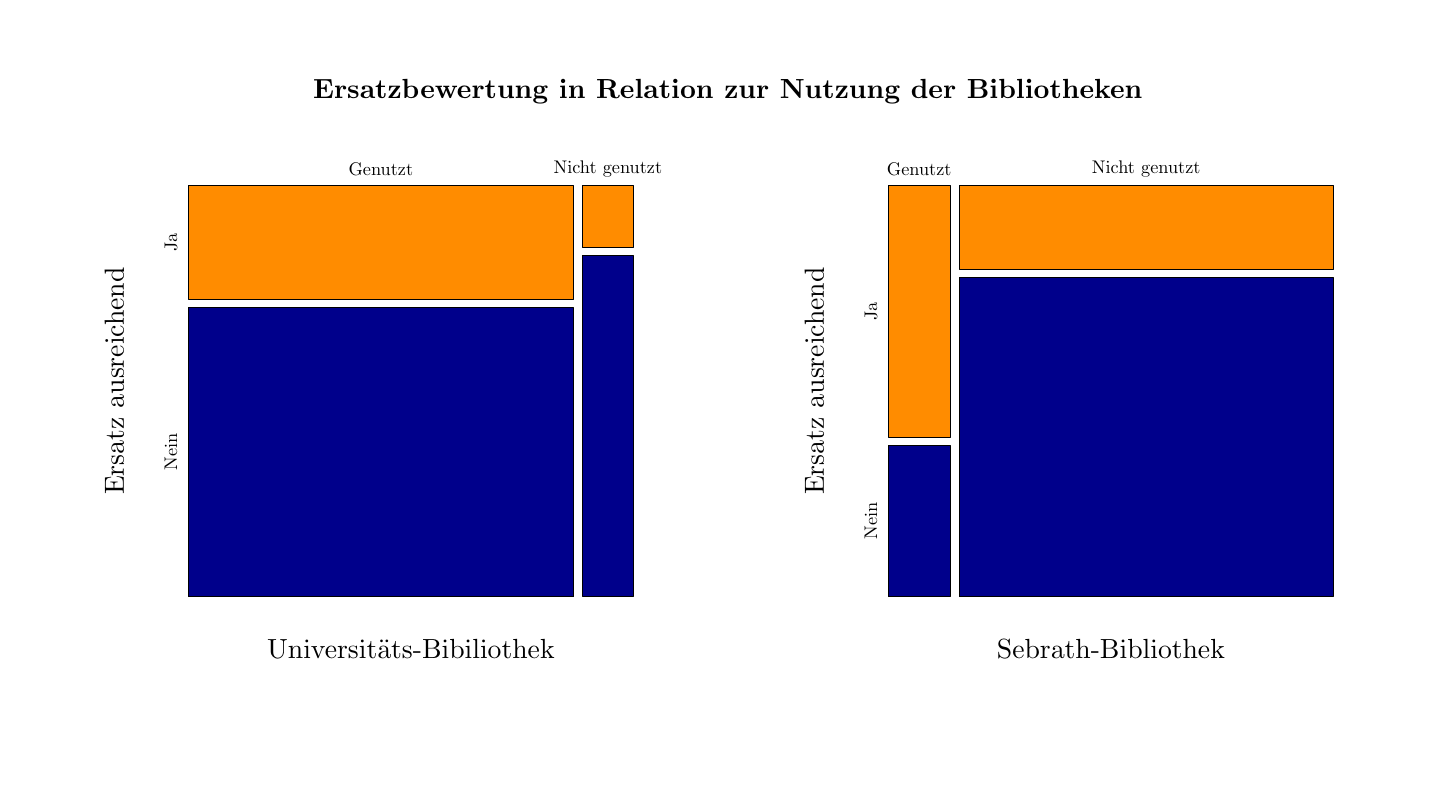
\begin{tikzpicture}[x=1pt,y=1pt]
\definecolor{fillColor}{RGB}{255,255,255}
\path[use as bounding box,fill=fillColor,fill opacity=0.00] (0,0) rectangle (505.89,267.40);
\begin{scope}
\path[clip] (  0.00,  0.00) rectangle (252.94,267.40);
\definecolor{drawColor}{RGB}{0,0,0}

\node[text=drawColor,anchor=base,inner sep=0pt, outer sep=0pt, scale=  1.20] at (138.47,238.66) {\bfseries  };

\node[text=drawColor,anchor=base,inner sep=0pt, outer sep=0pt, scale=  1.00] at (138.47, 39.60) {Universitäts-Bibiliothek};

\node[text=drawColor,rotate= 90.00,anchor=base,inner sep=0pt, outer sep=0pt, scale=  1.00] at ( 34.80,139.70) {Ersatz ausreichend};
\end{scope}
\begin{scope}
\path[clip] (  0.00,  0.00) rectangle (505.89,267.40);
\definecolor{drawColor}{RGB}{0,0,0}

\node[text=drawColor,anchor=base,inner sep=0pt, outer sep=0pt, scale=  0.66] at (127.63,213.94) {Genutzt};

\node[text=drawColor,anchor=base,inner sep=0pt, outer sep=0pt, scale=  0.66] at (209.66,214.58) {Nicht genutzt};

\node[text=drawColor,rotate= 90.00,anchor=base,inner sep=0pt, outer sep=0pt, scale=  0.66] at ( 53.97,189.76) {Ja};

\node[text=drawColor,rotate= 90.00,anchor=base,inner sep=0pt, outer sep=0pt, scale=  0.66] at ( 53.97,114.02) {Nein};
\end{scope}
\begin{scope}
\path[clip] ( 49.20, 61.20) rectangle (227.75,218.20);
\definecolor{drawColor}{RGB}{0,0,0}
\definecolor{fillColor}{RGB}{255,140,0}

\path[draw=drawColor,line width= 0.4pt,line join=round,line cap=round,fill=fillColor] ( 57.96,169.18) --
	(197.29,169.18) --
	(197.29,210.34) --
	( 57.96,210.34) --
	cycle;
\definecolor{fillColor}{RGB}{0,0,139}

\path[draw=drawColor,line width= 0.4pt,line join=round,line cap=round,fill=fillColor] ( 57.96, 61.83) --
	(197.29, 61.83) --
	(197.29,166.21) --
	( 57.96,166.21) --
	cycle;
\definecolor{fillColor}{RGB}{255,140,0}

\path[draw=drawColor,line width= 0.4pt,line join=round,line cap=round,fill=fillColor] (200.51,187.95) --
	(218.81,187.95) --
	(218.81,210.34) --
	(200.51,210.34) --
	cycle;
\definecolor{fillColor}{RGB}{0,0,139}

\path[draw=drawColor,line width= 0.4pt,line join=round,line cap=round,fill=fillColor] (200.51, 61.83) --
	(218.81, 61.83) --
	(218.81,184.98) --
	(200.51,184.98) --
	cycle;
\end{scope}
\begin{scope}
\path[clip] (252.94,  0.00) rectangle (505.89,267.40);
\definecolor{drawColor}{RGB}{0,0,0}

\node[text=drawColor,anchor=base,inner sep=0pt, outer sep=0pt, scale=  1.20] at (391.42,238.66) {\bfseries  };

\node[text=drawColor,anchor=base,inner sep=0pt, outer sep=0pt, scale=  1.00] at (391.42, 39.60) {Sebrath-Bibliothek};

\node[text=drawColor,rotate= 90.00,anchor=base,inner sep=0pt, outer sep=0pt, scale=  1.00] at (287.75,139.70) {Ersatz ausreichend};
\end{scope}
\begin{scope}
\path[clip] (  0.00,  0.00) rectangle (505.89,267.40);
\definecolor{drawColor}{RGB}{0,0,0}

\node[text=drawColor,anchor=base,inner sep=0pt, outer sep=0pt, scale=  0.66] at (322.16,213.94) {Genutzt};

\node[text=drawColor,anchor=base,inner sep=0pt, outer sep=0pt, scale=  0.66] at (404.20,214.58) {Nicht genutzt};

\node[text=drawColor,rotate= 90.00,anchor=base,inner sep=0pt, outer sep=0pt, scale=  0.66] at (306.92,164.86) {Ja};

\node[text=drawColor,rotate= 90.00,anchor=base,inner sep=0pt, outer sep=0pt, scale=  0.66] at (306.92, 89.12) {Nein};
\end{scope}
\begin{scope}
\path[clip] (302.14, 61.20) rectangle (480.69,218.20);
\definecolor{drawColor}{RGB}{0,0,0}
\definecolor{fillColor}{RGB}{255,140,0}

\path[draw=drawColor,line width= 0.4pt,line join=round,line cap=round,fill=fillColor] (310.90,119.38) --
	(333.42,119.38) --
	(333.42,210.34) --
	(310.90,210.34) --
	cycle;
\definecolor{fillColor}{RGB}{0,0,139}

\path[draw=drawColor,line width= 0.4pt,line join=round,line cap=round,fill=fillColor] (310.90, 61.83) --
	(333.42, 61.83) --
	(333.42,116.41) --
	(310.90,116.41) --
	cycle;
\definecolor{fillColor}{RGB}{255,140,0}

\path[draw=drawColor,line width= 0.4pt,line join=round,line cap=round,fill=fillColor] (336.64,180.02) --
	(471.75,180.02) --
	(471.75,210.34) --
	(336.64,210.34) --
	cycle;
\definecolor{fillColor}{RGB}{0,0,139}

\path[draw=drawColor,line width= 0.4pt,line join=round,line cap=round,fill=fillColor] (336.64, 61.83) --
	(471.75, 61.83) --
	(471.75,177.05) --
	(336.64,177.05) --
	cycle;
\end{scope}
\begin{scope}
\path[clip] (  0.00,  0.00) rectangle (505.89,267.40);
\definecolor{drawColor}{RGB}{0,0,0}

\node[text=drawColor,anchor=base west,inner sep=0pt, outer sep=0pt, scale=  1.00] at (103.17,241.74) {\bfseries Ersatzbewertung in Relation zur Nutzung der Bibliotheken};
\end{scope}
\end{tikzpicture}
